\documentclass[a4paper]{report}
% Shared preamble for the English probability and statistics documents.
% Based on the original course preamble. Compile with pdfLaTeX.
\usepackage[top=1.5cm,bottom=2cm,left=2cm,right=2cm]{geometry}
\usepackage[T1]{fontenc}
\usepackage{lmodern}
\usepackage[utf8]{inputenc}
\usepackage[english]{babel}

\usepackage{amsmath}
\usepackage{amssymb}
\usepackage{amsthm}
\usepackage{mathrsfs}
\usepackage{mathtools}
\usepackage{etoolbox}
\usepackage{tikz}
\usetikzlibrary{shapes.multipart,arrows.meta}
\usepackage{xcolor}
\usepackage{enumerate}
\usepackage[shortlabels]{enumitem}
\usepackage{hyperref}
\usepackage{version}
\usepackage{bbold}
\usepackage{fontawesome5}
\usepackage{fancyhdr}
\lfoot{}
\usepackage{natbib}
\usepackage{graphicx}
\usepackage{pdfpages}
\usepackage{authblk}
    
\usepackage{blindtext}
\usepackage{multicol}
\usepackage{collcell}
\usepackage{wrapfig}
\usepackage{blkarray}
\usepackage{cancel}
\usepackage{appendix}
\usepackage{float}
\makeatletter
\input{tex/assets/slashbox.sty}
\makeatother
\hypersetup{unicode,colorlinks,citecolor=red,filecolor=black,
  linkcolor=red,urlcolor=cyan}
\setlength{\columnsep}{1cm}
\pagenumbering{gobble}

\def\numtext#1{%
  \ifcase#1\or one\or two\or three\or four\or five\or six\or seven\or eight\or nine\or ten\or
  eleven\or twelve\or thirteen\or fourteen\or fifteen\or sixteen\or seventeen\or eighteen\or nineteen\or twenty\or Lots\fi}

\newcommand{\Byte}[1]{%
  \def\nodecontents{}%
  \foreach[count=\l] \k in {#1} {\xappto{\nodecontents}{\noexpand\nodepart{\numtext{\l}}\k}}%
  \node[rectangle split,rectangle split parts=8,rectangle split horizontal,draw] at (2,2){\nodecontents};}

\newcommand{\D}{{\mathrm{d}}}
\newcommand{\cE}{{\mathcal{E}}}
\newcommand{\cG}{{\mathcal{G}}}
\newcommand{\cX}{{\mathcal{X}}}
\newcommand{\cY}{{\mathcal{Y}}}
\newcommand{\cB}{{\mathcal{B}}}
\newcommand{\cF}{{\mathcal{F}}}
\newcommand{\cO}{{\mathcal{O}}}
\newcommand{\cS}{{\mathcal{S}}}
\newcommand{\cT}{{\mathcal{T}}}
\newcommand{\given}{\, \big| \,}
\newcommand{\cL}{{\mathscr{L}}}
\newcommand{\cD}{{\mathcal{D}}}
\newcommand{\cA}{{\mathscr{A}}}
\newcommand{\cP}{{\mathscr{P}}}
\newcommand{\cR}{{\mathscr{R}}}
\newcommand{\A}{{\mathcal A}}
\newcommand{\one}{\mathbb{1}}
\newcommand{\mathbbm}[1]{\mathbb{#1}}

\providecommand{\C}{}
\renewcommand{\C}{\mathbb C}
\newcommand{\R}{\mathbb R}
\newcommand{\Q}{\mathbb Q}
\newcommand{\N}{\mathbb N}
\newcommand{\T}{\mathbb T}
\newcommand{\F}{\mathbb F}
\renewcommand{\P}{\mathbb P}
\newcommand{\Z}{\mathbb Z}
\newcommand{\E}{\mathbb {E}}
\newcommand{\Pbb}[1]{\P\left( #1\right)}
\newcommand{\Ebb}[1]{\E\left[ #1\right]}

\newcommand{\lb}{\left (}
\newcommand{\rb}{\right )}
\newcommand{\lbb}{\left [}
\newcommand{\rbb}{\right ]}
\newcommand{\labs}{\left |}
\newcommand{\rabs}{\right |}
\newcommand{\lbrb}[1]{\lb #1 \rb}
\newcommand{\lbbrbb}[1]{\lbb#1\rbb}
\newcommand{\labsrabs}[1]{\labs#1\rabs}
\newcommand{\lbbrb}[1]{\lbb#1\rb}
\newcommand{\lbrbb}[1]{\lb#1\rbb}
\newcommand{\langlerangle}[1]{\langle#1\rangle}
\newcommand{\lbcurly}{\{}
\newcommand{\rbcurly}{\}}
\newcommand{\curly}[1]{\lbcurly#1\rbcurly}
\newcommand{\abs}{\labsrabs}
\newcommand{\ind}[1]{1_{#1}}
\newcommand{\indep}{\perp \!\!\! \perp}
\renewcommand{\d}{\, \mathrm{d}}

\newtheorem{theorem}{Theorem}
\newtheorem{problemCnt}{Lemma}
\theoremstyle{definition}
\newtheorem{problem}[problemCnt]{Problem}
\newtheorem{problembook}[problemCnt]{\faBook \,  Problem}
\newtheorem{problempencil}[problemCnt]{\faPencil* \,  Problem}
\newtheorem{problemstar}[problemCnt]{\faStar\,  Problem}
\newtheorem{problemstarpencil}[problemCnt]{\faStar \, \faPencil* \,   Problem}
\newtheorem{probleminteresting}[problemCnt]{\faSmile[regular] \,   Problem}
\newtheorem{solution}{Solution}

\newcommand{\fwcell}[1]{\makebox[\arraystretch\normalbaselineskip]{$#1$}}
\newenvironment{enumeratei}{\begin{enumerate}[(i)]}{\end{enumerate}}
\newenvironment{enumeratea}{\begin{enumerate}[(a)]}{\end{enumerate}}
\newenvironment{enumeraten}{\begin{enumerate}[\upshape 1.]}{\end{enumerate}}

% Compatibility helpers needed by a few files in the combined archive.
\AtBeginDocument{\noindent{\footnotesize English translation prepared with ChatGPT (OpenAI, GPT-6), 26 October 2026, for translation of the Bulgarian text into English and LaTeX formatting.
The Bulgarian originals remain the reference; translation may contain errors.}\par\smallskip}
\newcommand{\MissingGraphic}[1]{%
  \begin{center}\fbox{\parbox{0.82\linewidth}{\centering Missing source image: \texttt{#1}}}\end{center}}



\begin{document}
\noindent Computer Science, 12 June 2025 \hfill Examination problems
\hrulefill
\begin{it}The exact grading formula depends on the results. As an approximation, use 2 + the number of points. Time allowed: 4 hours. Good luck!\end{it}
\begin{problem}
\begin{enumerate}
\item Ten cards carry the letters of the Bulgarian word for probability, transliterated as V, E, R, O, YA, T, N, O, S, T. Here YA represents one Cyrillic letter and is a vowel.
\begin{enumerate}
\item (0.25 points) Find the probabilities of: $A$, drawing five letters without replacement from which the name STOYAN (S,T,O,YA,N) can be formed; $B$, drawing three consonants with/without replacement; $C$, drawing four letters without replacement with equal numbers of vowels and consonants.
\item (0.25 points) Let $X,Y$ count vowels and consonants, respectively, in seven random draws with replacement. Find $\mathrm{Cor}(X,Y)$.
\end{enumerate}
\item (0.5 points) Three radio signals are sent successively and independently, with reception probabilities $1/2,1/3,1/4$. Let $X$ count received signals. Find the expectation and distribution of $\xi$. Communication succeeds with probability 0.2, 0.6 or 1 if one, two or three signals are received, respectively. What is its overall probability of success?
\item (0.5 points) Repeatedly roll a standard die. Let $X$ count rolls until the first six and $Y$ rolls until all faces have appeared. Find their probability generating functions and expectations.
\end{enumerate}
\end{problem}
\begin{problem}
A battery's lifetime is normal with mean 300 hours and standard deviation 20.
\begin{enumerate}
\item (0.25 points) What lifetime will 98\% of batteries exceed?
\item (0.25 points) A device with four batteries operates while at least one remains charged. What is the probability it works for at least 350 hours?
\end{enumerate}
\end{problem}
\begin{problem} (0.5 points)
Let $X$ be the age of a car involved in an accident and $Y$ the duration of its insurance before the accident, in years. Their joint density is $f(x,y)=c(10-xy^2)$ for $2\leq x\leq10$, $0\leq y\leq1$. What is the mean age of an accident-involved car? Find the probability that it was first insured less than half a year before the accident.
\end{problem}
\begin{problem}
\begin{enumerate}
\item (0.5 points) In a physics experiment, Galya sends a particle at constant speed around a circular groove of radius 1 and places a screen of length 2 at distance 1 from it, as shown. At a random time, the particle leaves tangentially. Find the probability that it hits the screen.
\begin{figure}[h]\centering
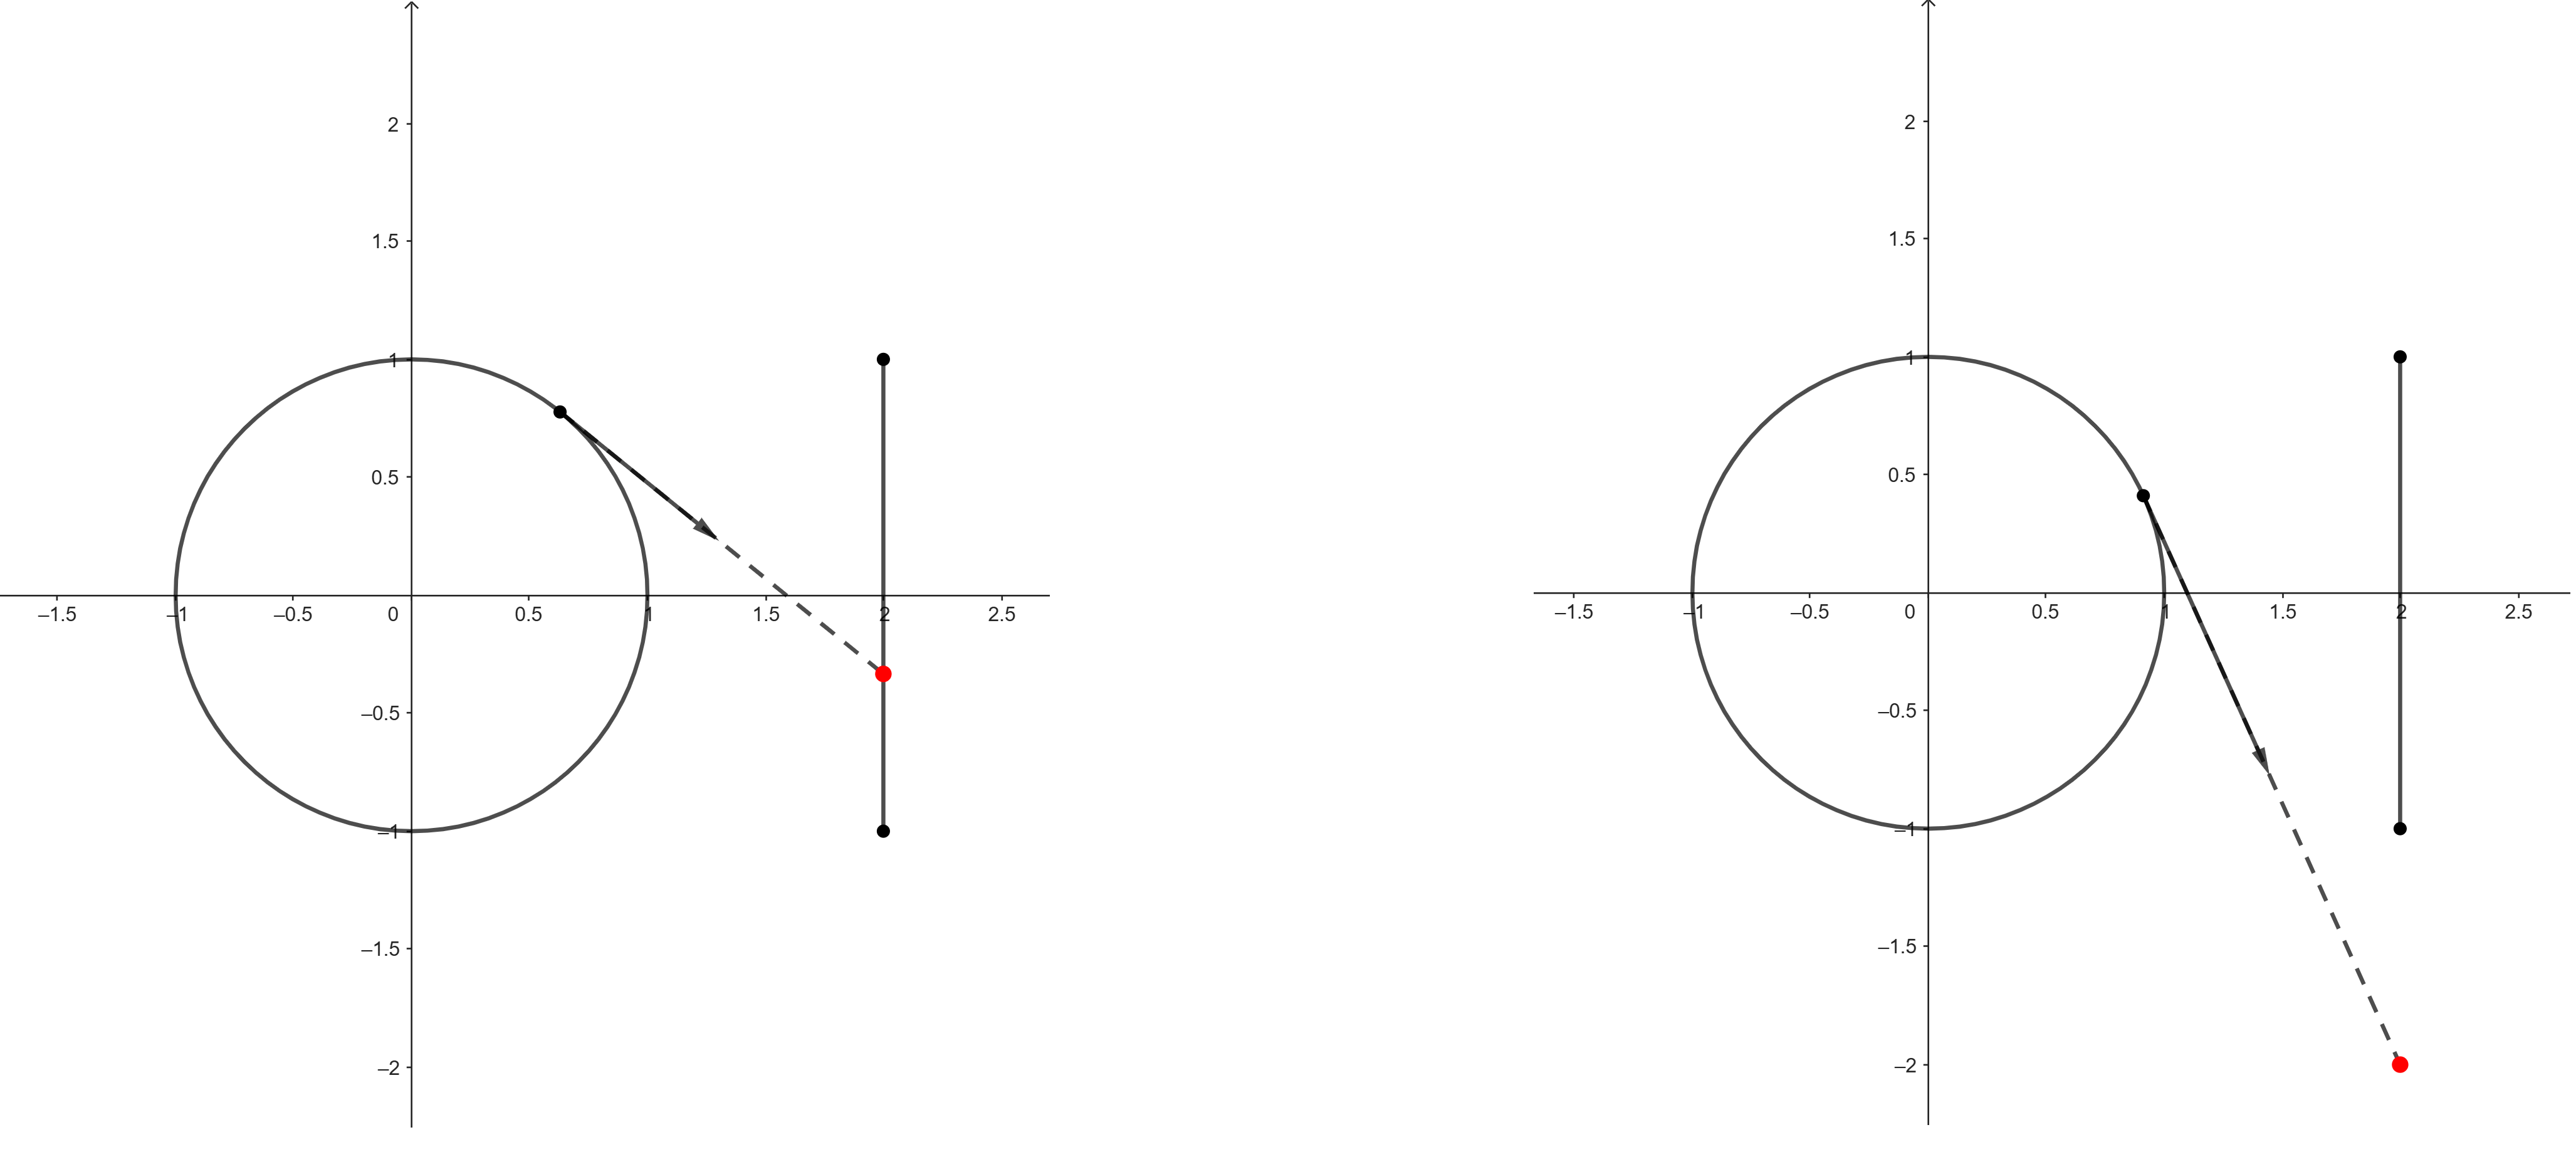
\includegraphics[scale=0.075]{tex/assets/prob-stat/computer-science-2/KN_IZPIT_1.png}
\caption{Diagram for the particle-and-screen problem.}
\end{figure}
\item (0.5 points) Let $X,Y$ be independent $\mathcal N(0,1)$. For fixed $\theta$, set $U=X\cos\theta+Y\sin\theta$ and $V=-X\sin\theta+Y\cos\theta$. Show that $U,V$ are independent and find their distributions.
\item (0.5 points) A shot at a circular target centred at the origin lands at independent $N(0,1)$ coordinates.
\begin{enumerate}
\item (0.5 points) Prove that its distance $R=\sqrt{X^2+Y^2}$ from the centre has density $f_R(r)=re^{-r^2/2}$, $r\geq0$.
\item (0.5 points) Show that $\E[R]=\sqrt{\pi/2}$, its median is $\sqrt{\ln4}$, and its mode is 1.
\end{enumerate}
\end{enumerate}
\end{problem}
\end{document}
